\documentclass[12pt,spanish,fleqn,openany,letterpaper,pagesize]{scrbook}

\usepackage[utf8]{inputenc}
\usepackage[spanish]{babel}
\usepackage{fancyhdr}
\usepackage{epsfig}
\usepackage{epic}
\usepackage{eepic}
\usepackage{amsmath}
\usepackage{threeparttable}
\usepackage{amscd}
\usepackage{here}
\usepackage{graphicx}
\usepackage{lscape}
\usepackage{tabularx}
\usepackage{subfigure}
\usepackage{longtable}


\usepackage{rotating} %Para rotar texto, objetos y tablas seite. No se ve en DVI solo en PS. Seite 328 Hundebuch
                        %se usa junto con \rotate, \sidewidestable ....


\renewcommand{\theequation}{\thechapter-\arabic{equation}}
\renewcommand{\thefigure}{\textbf{\thechapter-\arabic{figure}}}
\renewcommand{\thetable}{\textbf{\thechapter-\arabic{table}}}


\pagestyle{fancyplain}%\addtolength{\headwidth}{\marginparwidth}
\textheight22.5cm \topmargin0cm \textwidth16.5cm
\oddsidemargin0.5cm \evensidemargin-0.5cm%
\renewcommand{\chaptermark}[1]{\markboth{\thechapter\; #1}{}}
\renewcommand{\sectionmark}[1]{\markright{\thesection\; #1}}
\lhead[\fancyplain{}{\thepage}]{\fancyplain{}{\rightmark}}
\rhead[\fancyplain{}{\leftmark}]{\fancyplain{}{\thepage}}
\fancyfoot{}
\thispagestyle{fancy}%


\addtolength{\headwidth}{0cm}
\unitlength1mm %Define la unidad LE para Figuras
\mathindent0cm %Define la distancia de las formulas al texto,  fleqn las descentra
\marginparwidth0cm
\parindent0cm %Define la distancia de la primera linea de un parrafo a la margen

%Para tablas,  redefine el backschlash en tablas donde se define la posici\'{o}n del texto en las
%casillas (con \centering \raggedright o \raggedleft)
\newcommand{\PreserveBackslash}[1]{\let\temp=\\#1\let\\=\temp}
\let\PBS=\PreserveBackslash

%Espacio entre lineas
\renewcommand{\baselinestretch}{1.1}

%Neuer Befehl f\"{u}r die Tabelle Eigenschaften der Aktivkohlen
\newcommand{\arr}[1]{\raisebox{1.5ex}[0cm][0cm]{#1}}

%Neue Kommandos
\usepackage{Befehle}


%Trennungsliste
\hyphenation {Reaktor-ab-me-ssun-gen Gas-zu-sa-mmen-set-zung
Raum-gesch-win-dig-keit Durch-fluss Stick-stoff-gemisch
Ad-sorp-tions-tem-pe-ra-tur Klein-schmidt
Kohlen-stoff-Mole-kular-siebe Py-rolysat-aus-beu-te
Trans-port-vor-gan-ge}


\begin{document}

\section{Epidemiología Panorámica}

\justifying


\par La \textit{Teledetección} se define como el proceso de adquirir
  información acerca de un objeto, área o fenómeno desde la distancia.
  Un sensor remoto es un instrumento capaz de realizar percepción remota, por lo
  que en esta amplia definición caben desde los ojos hasta los
  radiotelescopios.

\par Existen dos grandes tipos de sensores remotos (SR): activos y pasivos.
  Los activos son aquellos que obtienen la información generando su propia energía
  mientras que los pasivos dependen de una fuente externa, que en la Tierra
  principalmente proviene del Sol. Hasta el día de hoy, los más usados son los
  sensores pasivos dado que permiten medir la magnitud de la radiación electromagnética
  reflejada e irradiada desde la superficie de la Tierra y de la atmósfera y,
  de esta manera, derivar información sobre las condiciones de la superficie \cite{cami_tartagal}.


\par Los SR más utilizados y con mayor cantidad de aplicaciones son los que se
  encuentran a bordo de satélites que orbitan sobre la Tierra, bien sea
  en órbitas geoestacionarias\footnote{Están en altitudes entre 23000 y 40000 km,
  sobre la franja ecuatorial y viaja a la misma velocidad de rotación de la Tierra
  por lo que siempre están fijos sobre un punto determinado de la superficie terrestre},
  u órbitas polares, los cuales pasan repetidamente por diferentes áreas
  de la Tierra mientras están orbitando alrededor del planeta a altitudes menores.


\par Las tecnologías relacionadas al ámbito aeroespacial dieron lugar a programas
  que integran estas tecnologías con,
  por ejemplo, la agricultura, salud pública, geología y las ciencias forestales.
  A su vez, la información obtenida por dichos SR se puede aplicar a estudios
  entomológicos\footnote{De insectos}, debido a que ellos proveen gran cantidad
  y diversidad de información sobre la cobertura de la Tierra: características
  de la vegetación, cuerpos de agua, temperaturas, entre otras. Ésta, también es
  información sobre el hábitat de insectos y artrópodos vectores \cite{ndwi_erffectiveness, data_driven_prediction},
  y, por lo tanto, de acuerdo a la teoría de Pavlovsky \cite{nidality} en la que
  expone la correlación entre el hábitat y enfermedades transmitidas por vectores,
  los datos de los SR se pueden utilizar como fuente de información sobre la
  distribución espacio-temporal de dichas afecciones.


\par Con la acumulación de datos registrados por sensores remotos desde los años
  70 existen series temporales que permiten realizar varios tipos de análisis con
  relevancia para la transmisión de la enfermedad de Dengue y otras
  enfermedades de transmisión vectorial.
  Entre ellas, series temporales de imágenes de mediana resolución espacial
  permiten analizar en perspectiva histórica los cambios de uso y cobertura del
  terreno, proceso que habitualmente tiene vinculación con cambios en la
  epidemiología de la enfermedad \cite{german_temporal}.
  A su vez, el deterioro de las condiciones de salud en el mundo, el avance significativo
  en el procesamiento de computadoras, la mejora en la adquisición de datos,
  la reducción de los costos de hardware y software y el desarrollo de tecnología
  de Sistemas de Información Geográfica (GIS) han llevado al lanzamiento
  de programas que apuntan a integrar SR / GIS en aplicaciones de salud
  \cite{tesis_riesgo_viral, tesis_gonza, espinosa_temporal, rs_public_health}.



\par El uso de técnicas de Teledetección para mapear la distribución de vectores y el riesgo
  de enfermedades ha tenido una gran evolución durante las últimas dos
  décadas. La complejidad de las técnicas va desde el uso de simples
  correlaciones entre las firmas espectrales de diferentes coberturas, usos del
  suelo y abundancia de especies \cite{spectral_spatial, potencial_use} hasta
  técnicas complejas que integran variables
  ambientales obtenidas de satélites con la biología de los vectores
  \cite{ndwi_erffectiveness, malaria_impact}.
  Estas técnicas se usan para desarrollar modelos predictivos de riesgo,
  los cuales principalmente se realizan a través de técnicas estadísticas de
  regresión logística y análisis discriminante, que dilucidan las asociaciones
  entre datos ambientales multivariados y los patrones de presencia o ausencia de
  vectores para así mapear los vectores o las enfermedades.
  Estos métodos son capaces de predecir la probabilidad “\textit{a posteriori}” de la
  presencia de la variable dependiente (vector o enfermedad), a partir de un
  grupo de variables independientes (datos de clima y cobertura de la tierra) y de esta
  forma pueden ser usados para hacer mapas de riesgo a partir de bases de datos.


% la vision panotamira de los problemas de este tipo esta vinculada con la
% el hecho de que dichos problemas dependen de un entorno no local
\par Cabe aclarar que la visión panorámica de los problemas de este tipo está
  vinculada con el hecho de que dependen de un entorno no local. Es por esta
  razón que resulta importante hablar acerca de la \textit{conectividad}
  \footnote{El grado en que el paisaje impide o facilita el movimiento
  entre las zonas de recursos \cite{landscape_connectivity}} de los paisajes.
  Las condiciones ambientales que determinan dicha conectividad
  para la disperción pueden variar en las distintas regiones y dependen de cómo
  el patógeno se dispersa biológicamente (e.j: dado un patógeno portado por
  vectores, el movimiento del insecto) o abióticamente (e.j: flujos de viento o agua).
  Por ejemplo, rios y corrientes pueden actuar como corredores de disperción que
  fomentan la propagación de la infección a través de paisajes heterogéneos
  para patógenos de plantas transmitidos por el agua, mientras que en otros
  sistemas, como las enfermedades zoonóticas de mamíferos terrestres, estos mismos
  cuerpos de agua pueden funcionar como barreras impidiendo el movimiento
  del huesped o del vector. Éstas condiciones se ven reflejadas en la
  Figura \ref{fig:paisajes_h} de \cite{landscape_epidemiology}.
  Notemos que en el caso de \textbf{a)}, la
  conectividad entre los sitios azules es mayor que la que se da entre éstos y
  los amarillos, y también entre ellos y los rojos, siendo que la distancia
  Euclidea entre los azules es mayor. Ésto ocurre porque el sitio rojo está del otro lado
  de la cordillera, la cual funciona como una barrera geográfica para la
  inoculación\footnote{Introducción de microorganismos vivos, muertos o atenuados,
  en un organismo de forma accidental o voluntaria.}, el huésped y/o la disperción
  del vector. En el caso \textbf{b)}, en cambio, se da la situación de un
  patosistema\footnote{Subsistema dentro del sistema agrícola caracterizado por el
  fenómeno de parasitismo. Está constituido por un hospedante susceptible,
  un patógeno virulento y un ambiente predispuesto a la enfermedad} acuático, en
  donde la inoculación sucede a través del agua: los dos sitios amarillos son los
  más estrechamente conectados, a pesar de que están separados por una mayor
  distancia Euclidea que con otros, porque el sitio amarillo de abajo está localizado
  bajo una corriente que va desde el sitio amarillo de arriba.

  \begin{figure}
  \centering%
  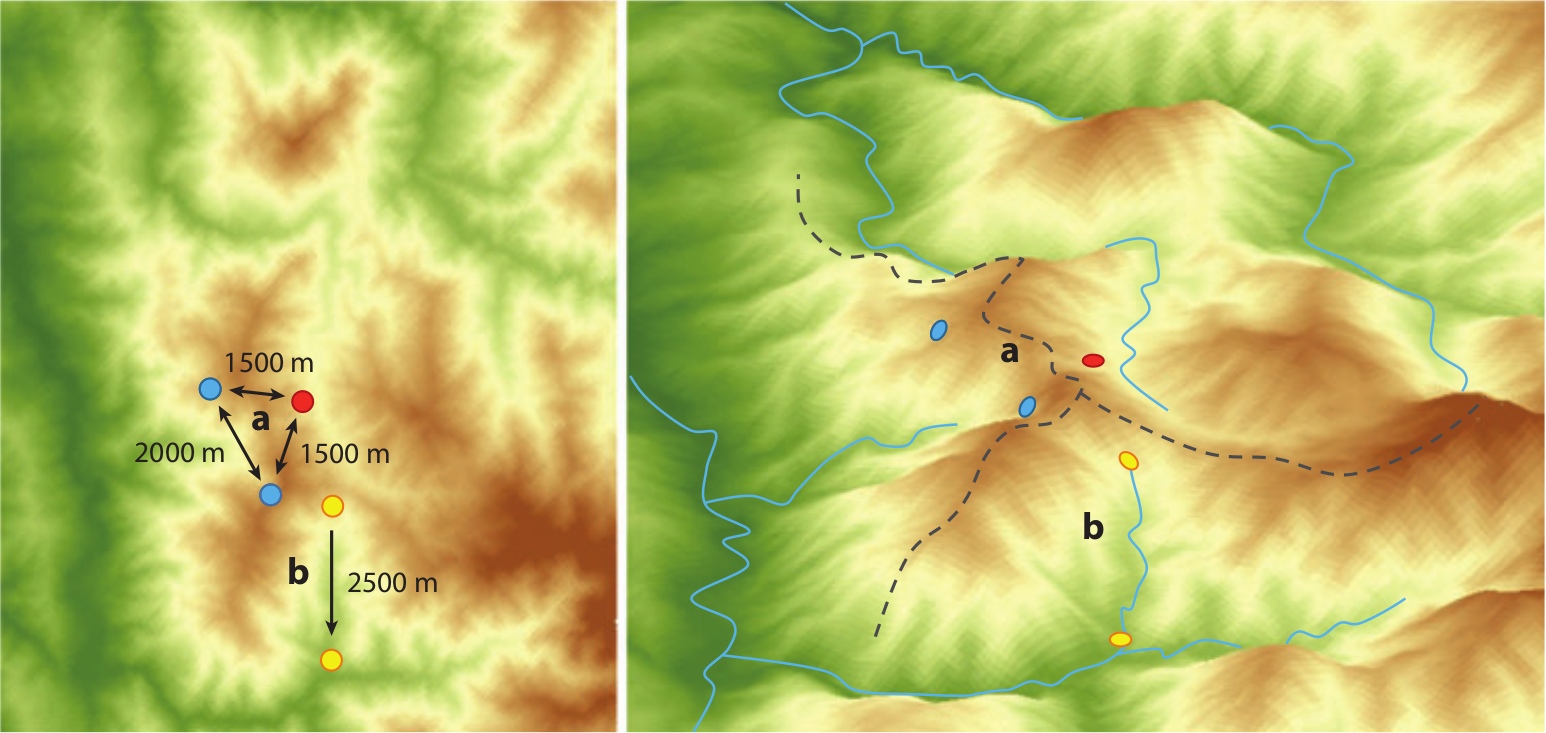
\includegraphics[width=1\textwidth]{images/paisajes_heterogeneos}%
  \caption{La propagación y persistencia a través de paisajes heterogéneos}\label{fig:paisajes_h}
  \end{figure}

% con un así se pega acá
  \par Así, la \textbf{\textit{Epidemiología Panorámica}}\cite{nidality, ostfeld_re_emerging}
  (EP) está estrechamente relacionada a su paralela ecológica, la Ecología
  Panorámica, una ciencia con inicios en los años 1930s que se dedica a estudiar
  las interacciones entre los ambientes y la vegetación \cite{landscape_ecology}.
  Sin embargo, los paisajes son espacial y temporalmente dinámicos.
  En simultáneo con el nacimiento de la ecología panorámica como una ciencia,
  Pavlosky estipula el concepto de \textit{nidalidad}\footnote{Se define como
  el foco de la infección. Además, Pavlosky, establece que los focos de
  enfermedades a microescala están determinados por todo el ecosistema \cite{nidality}}
  (o focalidad) de las enfermedades, donde los patógenos son asociados
  a paisajes (zonas) específicos. Un foco de infección contiene tres elementos
  críticos \cite{reisen_landscape}:
  \begin{enumerate}
    \item Vectores con capacidad de transmisión de la infección
    \item Vertebrados capaces de funcionar como reservorio de la infección
    \item Huéspedes susceptibles, como humanos o animales domésticos
  \end{enumerate}
  El concepto de \textit{focalidad} mezclado con la ecología panorámica
  llevó al nacimiento de la ciencia contemporánea
  \textbf{\textit{Epidemiología Panorámica}}, en la cual las enfermedades
  pueden ser asociadas a distintas características del paisaje o cómo
  la configuración entre el vector, el huésped y el patógeno se intersecan
  dado un clima permisivo para que ello suceda.

\par Por definición, la \textit{EP} integra conceptos y
  enfoques de la ecología vinculada a las enfermedades, con el análisis a
  macroescala de la ecología del paisaje. La intersección de estas perspectivas
  nos habilita a entender cómo es que la configuración espacial y las
  características de la composición del paisaje afectan a los procesos
  epidemiológicos a lo largo y ancho de las áreas geográficas que se
  extienden más allá de los procesos que operan localmente dentro de una sola comunidad.
  Así, la \textit{EP} es más que simplemente establecer
  sectores en el territorio y examinar diferencias en condiciones locales de
  factores bióticos y abióticos entre distintos lugares; la clave es obtener
  información sobre la distribución geográfica de la enfermedad y comprender
  cómo las interrelaciones de los paisajes influencian las interacciones entre
  individuos susceptibles e infectados.

\par La EP ha sido aplicada en gran variedad de estudios sobre vectores de
  enfermedades (28-37). A nivel global, se pueden encontrar contribuciones en esta área
  [32, 33, 34] también con algunas experiencias de herramientas operativas [35].
  A su vez, muchos estudios interdisciplinarios fueron llevados a cabo en
  latinoamérica enfocados en la generación de modelos predictivos de riesgo,
  espaciales y temporales, basados en condiciones ambientales derivadas de
  información satelital [24, 25, 26, 27].
  Por ejemplo, en México, Dumonteil y Gourbiere (38)
  estudiaron la relación entre la distribución de la especie Triatoma dimidiata
  y factores bioclimáticos, para de esta forma desarrollar un modelo predictivo de
  la abundancia domiciliaria por esta especie y las tasas de infección
  por T. cruzi. Estas predicciones se usaron para construir el primer mapa de
  riesgo de transmisión en la península de Yucatán hallándose que la abundancia de T.
  dimidiata se asocia de forma positiva (por análisis de regresión de Poisson)
  con los cultivos, pastos, precipitación, humedad relativa y la temperatura
  máxima. En particular, en Argentina existen varias experiencias en esta
  dirección, [28, 29, 30] abordan el problema de la epidemia del Dengue dando
  herramientas operacionales [31].

\par Por ejemplo, en 2011, Argentina comenzó a desarrollar un proyecto operacional
  (Sistema de Alerta Temprana de Salud, HEWS), útil tanto para las autoridades de
  salud como para los investigadores.
  Básicamente, HEWS es un mapeo de riesgo dinámico del dengue para todas las
  ciudades del país. En este producto, cada ciudad es representada por un punto
  al que se le asigna un valor de riesgo para cada año, basado en tecnología
  geoespacial. El trabajo fue realizado en un contexto interdisciplinario e
  interinstitucional. En este sistema [13], el riesgo se evalúa en cuatro componentes que son: el
  entomológico, el viral, el componente relacionado con las actividades de
  control y finalmente el ambiental. Mientras que los tres primeros componentes
  se generan con el aporte de información de los agentes de salud que trabajan en cada
  ciudad, el cuarto se evalúa a partir de datos satelitales.
  Específicamente el componente ambiental, en la versión inicial del sistema, se
  evalúa con una probabilidad estacionaria de presencia de vectores (igual para
  todo el tiempo) más un componente relacionado con el número de ciclos virales,
  que son una función de la temperatura, y así es diferente para cada ciudad y
  para cada año. El mapa de probabilidad de presencia de especie (modelo de nicho)
  es claramente una gran simplificación y se puede mejorar en base a datos
  satelitales continuos del medio ambiente. Variables como precipitación y
  temperatura, han demostrado, con una variabilidad local, influenciar el
  desarrollo de mosquitos, su supervivencia y actividad de
  oviposición\footnote{Proceso de implantación o difusión de huevos plenamente
  desarrollados a partir del cuerpo de la hembra} y por ende la abundancia de vectores.

\par Otro ejemplo a destacar en la utilización de éstas técnicas en Argentina es
  el trabajo de German y colaboradores \cite{german_temporal}, en 2017.
  En él desarrollan una metodología completa
  para generar modelos de manera automática y basada en información de libre
  acceso. En particular German \cite{german_temporal} utiliza productos del sensor (MODIS) a bordo
  del satélite Terra y Aqua, pues es uno de los más adecuados para esta
  aplicación particular, debido a su resolución temporal, espectral y espacial.
  MODIS proporciona un conjunto de productos pre-procesados y de libre acceso \cite{terra_aqua_modis}.
  Específicamente, los productos de vegetación (índice de vegetación de diferencia
  normalizada) y temperatura (temperatura de la superficie terrestre) derivados
  de MODIS son ejemplos de variables de percepción remota utilizadas
  en aplicaciones de epidemiologia [13], [22] incorporadas en [20]. Otra variable
  ambiental obtenida de satélite que es relevante e incorporada, es el
  \textit{Índice de Agua de Diferencia Normalizada} (NDWI) que evalúa de alguna
  forma el contenido de agua de la cubierta. Adicionalmente el trabajo de German
  incorpora una estimación de la precipitación desde el espacio a partir de las
  misiones (TRMM) y (GPM) [23].
  Utilizando los datos mencionados como variables independientes,
  desarrollaron modelos temporales de pronóstico de oviposición de \textit{Aedes Aegypti}
  usando un método lineal multivariado. En su trabajo, mencionan que
  realizaron muchos métodos con distintos períodos de tiempo y que se llegó a
  construir uno con una buena capacidad de
  predicción ($R^{2} = 0.7 $ utilizando 11 variables ambientales independientes en total)

\end{document}
